\documentclass{report}
\usepackage[utf8]{inputenc}
\usepackage[a4paper,margin=3cm,top=2cm]{geometry}
\usepackage{graphicx}
% graphics
\usepackage{tikz}
\usepackage{graphicx}
\usepackage{booktabs}
\usepackage{dirtree}
\usepackage{float}
\usepackage{tabularx}
\usepackage[indentafter]{titlesec}
\usepackage{xlop}
\usepackage{caption,subcaption}
\usepackage{setspace}
%listings
\usepackage{xcolor}
\usepackage{listings}
\lstdefinestyle{verilog}{
	backgroundcolor=\color{gray!10!white},
	basicstyle=\footnotesize\ttfamily,
	breaklines=true,
	commentstyle=\color{gray},
	escapeinside={~}{~},
	frame=single,
	keywordstyle=\color{blue},
	language=verilog,
	numbers=left,
	numbersep=5pt,
	showstringspaces=false,   
	numberstyle=\tiny\color{gray},
	rulecolor=\color{gray},
	stringstyle=\color{purple},
	tabsize=4}
\lstnewenvironment{code}{\lstset{style=verilog}\latin}{\endlatin}

\newcommand{\co}[1]{\lr{\lstset{style=verilog}\lstinline{#1}}}


\usepackage{fancyhdr}
\pagestyle{fancy}
\fancyhf{}
\fancyhead[LE,RO]{\leftmark}
\fancyhead[RE,LO]{مستند پروژه طراحی سیستم‌های دیجیتال}
\fancyfoot[LE,RO]{\thepage}

\onehalfspacing
% persian
\usepackage[extrafootnotefeatures,localise]{xepersian}
\settextfont[
Scale = 1.2]{XB Zar}
\setlatintextfont[Scale=1.2,
 BoldFont={LiberationSerif-Bold.ttf}, 
 ItalicFont={LiberationSerif-Italic.ttf}]{LiberationSerif-Regular.ttf}
 
\begin{document}

\begin{titlepage}
\newcommand{\HRule}{\rule{\linewidth}{0.1mm}} 
\center % Center everything on the page
 
%---------------------------------------------------------------------------------
%	HEADING SECTIONS (Enter the Homework/assignment No., only)
%---------------------------------------------------------------------------------
    \textsc{\Large دانشکده مهندسی کامپیوتر}\\[0.5cm] % heading course Number
    \textsc{\Large طراحی سیستم‌های دیجیتال}\\[0.5cm] % heading course name
    \textsc{\large مستند پروژه}\\[0.5cm] % Minor heading
%---------------------------------------------------------------------------------
%	TITLE SECTION (Replace 'TITLE' with the Homework/assignment Name/title)
%---------------------------------------------------------------------------------

\HRule \\[0.4cm]
    { \huge \bfseries  بررسی الگوریتم درهم‌سازی skein}\\[0.1cm] % Title of your Homework/assignment
\HRule \\[1.5cm]
 
%\maketitle
\begin{minipage}{0.4\textwidth}
\begin{center}

 \large
    
    \emph{نگارندگان:}\\
    حسن سندانی\\
    محمد صالح سعیدی\\
    مریم حکاک\\
    محمد مهدی عرفانیان\\
    علی جندقی
    \end{center}
\end{minipage}
\vspace{10mm}

{\large \today}\\[1cm] % Date, change the \today to a set date if you want to be precise

\includegraphics{figs/sharif.png}% \\[0.5cm] % 
\vfill % Fill the rest of the page with white-space
\end{titlepage}
\tableofcontents
\chapter{مقدمه}
\noindent
\textbf{
\textit{
توضیحی اولیه مشتمل بر تعریف الگوریتم، نحوه کلی عملکرد الگوریتم، پایه‌های ریاضی، کاربردها و استانداردها
}
}
\pagebreak
\section{توضیح الگوریتم}
\par
الگوریتمی که در ادامهٔ این مستند شرح و توضیح آن آمده است الگوریتم درهم سازی 
\lr{skein}
یا 
\lr{skein hash function}
است. این الگوریتم از سری الگوریتم‌های درهم‌سازی امنیتی یا 
\lr{cryptographic hash function}
 و یکی از نامزدهای نهایی مسابقه انتخاب بهترین تابع درهم‌سازی 
 \lr{NIST}
 می‌باشد. این مسابقه برای انتخاب بهترین الگوریتم در‌هم‌سازی برای استاندارد جدید 
 \lr{SHA-3}
 برگزار شد. 
 طبق ادعای طراحان الگوریتم این الگوریتم می‌تواند در 
 \lr{6.1}
 کلاک در بایت داده‌ها را هش کند، که به این معنیست که در پردازندهٔ دوهسته‌ای
 \lr{64}
  بیتی با فرکانس پردازشی
\lr{3.1 GHz}
    می‌تواند با سرعت 
\lr{500}
  مگابایت بر ثانیه داده‌ها را هش کند. این مقدار سرعت تقریبا دوبرابر سرعت هش کردن دادهٔ الگوریتم 
  \lr{ SHA-512}
  است. همچنین با گزینه درخت درهم‌سازی که می‌تواند به صورت اختیازی در الگوریتم پیاده‌سازی شود می‌توان 	در پیاده‌سازی موازی الگوریتم سرعت را به بیش از این هم رساند. نکته دیگری که در مورد الگوریتم 
  \lr{skein}
  لازم به ذکر است این است که این الگوریتم پیاده‌سازی آسان و ساده‌ای دارد و فقط از سه عمل‌گر اصلی برای محاسبه هش استفاده می‌کند و نحوهٔ عملکرد الگوریتم به راحتی قابل به خاطرسپاری و یادگیری‌ست. 
  \par
  الگوریتم درهم‌سازی
  \lr{skein}
  برای حالت‌های ورودی ۲۵۶، ۵۱۲ و ۱۰۲۴ بایتی و هرمقداری خروجی پیاده‌سازی شده است که این خاصیت در انعطاف الگوریتم در حالت‌های مختلف بسیار حیاتی‌ست. 
  \\
  در پیاده‌سازی سخت‌افزاری نیز این الگوریتم قوی عمل می‌کند،‌برای پیاده‌سازی 
  \lr{skein-512}
  بر سخت‌افزار به حدود ۲۰۰ بایت فضای مموری نیاز داریم، برای 
  \lr{skein-256}
  این مفدار به حدود ۱۰۰ بایت کاهش پیاده می‌کند که این الگوریتم را به یک الگوریتم مناسب برای پیاده‌سازی‌های روی قطعات کوچک سخت‌افزاری تبدیل می‌کند، مثلا می‌توان از 
  \lr{skein-256}
  در پیاده‌سازی 
  \lr{smart card}
  استفاده کرد.
  \cite{skein}
 
  
  \subsection{مثال‌هایی از درهم‌سازی}

	\begin{itemize}
	
	\item \lr{Skein-256-256("")}\\
$c8877087da56e072870daa843f176e9453115929094c3a40c463a196c29bf7ba$
\item \lr{Skein-512-256("")}\\
$39ccc4554a8b31853b9de7a1fe638a24cce6b35a55f2431009e18780335d2621$
\item \lr{Skein-512-512("")}\\
$bc5b4c50925519c290cc634277ae3d6257212395cba733bbad37a4af0fa06af4$\\
$1fca7903d06564fea7a2d3730dbdb80c1f85562dfcc070334ea4d1d9e72cba7a$

	\end{itemize}
	
\section{مختصری دربارهٔ الگوریتم‌های درهم‌سازی امنیتی}
در دنیای امروز الگوریتم‌های درهم‌سازی امنیتی تقریبا در تمامی نقاط مختلفی که با اینترنت سر و کار دارند پیدا می‌شوند، بزرگ‌ترین کاربرد این الگوریتم‌ها ایجاد امضای دیجیتالی یا 
\lr{digital signature}
است که در ذخیرهٔ رمزهای عبور، اتصالات امنیتی به سرورها، مدیریت رمزنگاری‌ها و اسکن ویروس‌ها و بدافزارها به کار می‌رود، تقریبا تمامی پروتکل‌های امنیتی در دنیای اینترنت امروز بدون الگوریتم‌های درهم‌سازی امنیتی به سختی قابل پیاده‌سازی خواهند بود. 
\par
بزرگترین الگوریتم‌های درهم‌سازی امنیتی فعلی الگوریتم‌های خانواده 
\lr{SHA}
می‌باشند، الگوریتم‌های خانواده 
\lr{SHA}
به اختصار نام موارد زیر اند.
\begin{itemize}
\item
	\lr{SHA-0}
	\item
	\lr{SHA-1}
	\item
	\lr{SHA-256}
	\item
	\lr{SHA-512}
\end{itemize}
تمامی موارد بالا از روی الگوریتم‌های 
\lr{MD4} 	و
\lr{MD5}
اقتباس شده اند. 
در سال‌های اخیر کاستی‌ها و مشکلات امنیتی زیادی در الگوریتم‌های 
\lr{MD4, MD5, SHA-0, SHA-1}
یافت شدند اما هنوز باگ امنیتی بزرگی برای الگوریتم‌های 
\lr{SHA-256, SHA-512}
یافت نشده است اما به دلیل وابستگی زیاد صنعت و امنیت فعلی اطلاعات به الگوریتم‌های درهم‌سازی در سال ۲۰۱۲ 
تصمیم بر این شد تا جایگزین مناسب و جدیدی برای الگوریتم‌های 
\lr{SHA-256, SHA-512}
انتخاب شود تا در صورتی که این الگوریتم‌ها شکسته شدند به سرعت الگوریتم‌های جدید در قالب نام 
\lr{SHA-3}
جایگزین شوند. 
\section{هدف الگوریتم درهم‌سازی skein}	
هدف الگوریتم درهم‌سازی skein مانند دیگر الگوریتم‌های درهمسازی امنیتی ایجاد یک تابع برای درهم‌سازی داده‌های مختلف است به شکلی که ویژگی‌ها زیر برای آنان برقرار باشند.

\begin{itemize}
\item قطعی بودن:
به شکلی که به ازای ورودی یکسان مقدار در‌هم‌سازی با تکرار الگوریتم برابر باشد، مثلا با دادن ورودی "salam" به صورت متوالی به تابع مقدار هش تغییر نکند. 
\item یک طرفه بودن:
نتوان از مقدار خروحی مقدار ورودی را یافت. 
\item
یک به یک بودن:
نتوان دو ورودی پیدا کرد به شکلی که به ازای این دو ورودی مقدار خروجی مساوی شود.
\item حساس بودن:
با تغییر اندک در ورودی خروجی به شکل قابل ملاحظه‌ای تفییر کند تا مقدار هش قابل حدس زدن نباشد.
\item
سریع بودن: 
الگوریتم باید بتواند هش را در مدت زمانی کوتاهی حساب کند تا به کاربردی بودن برسد.

\end{itemize}


\section{نحوهٔ کلی عملکرد الگوریتم}
ایدهٔ اصلی الگوریتم بر ایجاد بلوک‌های زمزگذاری قابل تنظیم یا به زبان نویسندگان الگوریتم
\lr{tweakable block cipher}
بنا نهاده شده است؛ به صورت دقیق‌تر می‌توان گفت که
Skein 
از سه قسمت اصلی زیر تشکیل شده است و برای درهم‌سازی از ایشان استفاده می‌کند.
\begin{itemize}
\item
\lr{\textbf{Threefish}}\\
این قسمت یک بلوک رمزگذاری قابل تنظیم است که در هسته اصلی الگوریتم پیاده‌سازی شده است، این بلوک‌ها در سایزهای ۲۵۶، ۵۱۲، ۱۰۲۴ بیتی تعریف شده اند.
\item
\lr{\textbf{Unique Block Iteration (UBI)}}\\
\lr{UBI}
یک حالت زنجیری‌ست که با استفاده از بلوک قبلی به عنوان ورودی خود سعی در ایجاد یک الگوریتم فشرده‌سازی مخصوص ورودی می‌کند که بلوک ورودی با سایز دلخواه را به یک خروحی با سایز مشخص تبدیل کند.
\item
\lr{\textbf{Optional Argument System}}\\
این ویژگی به الگوریتم اجازه می‌دهد تا از تعدادی ویژگی اختیاری بدون تحمیل هزینه بیش از حد اجرایی استفاده کند. 
\cite{main_doc}
\end{itemize}
	
\begin{thebibliography}{1}


\bibitem{skein}{
\lr{
http://www.skein-hash.info/about\\
  }}
  
  \bibitem{main_doc}
  \lr{The Skein Hash Function Family\\
Version 1.3 — 1 Oct 2010\\
http://www.skein-hash.info/sites/default/files/skein1.3.pdf\\
}
  
\end{thebibliography}

\chapter{شبیه‌سازی}
\noindent
\textbf{
	\textit{
		توصیف روند شبیه‌سازی سخت‌افزار و گام‌های اجرایی، مشاهدهٔ ورودی‌ها و خروجی‌های اصلی و میانی، مقایسه با مقادیر حاصل از اجرای کد نرم‌افزاری (مدل طلایی)، توصیف مراحل اجزای الگوریتم به همراه شکل موج‌ها، نحوهٔ عملکرد 
		\lr{Testbench}
	}
}
\pagebreak

\section{توضیح روند شبیه‌سازی سخت‌افزار و گام‌های اجرایی}
برای شبیه‌سازی سخت‌افزاری کد 
\lr{verilog}
الگوریتم 
\lr{Skein}
را در محیط شبیه‌سازی 
\lr{Modelsim}
اجرا کردیم. گام‌های اجرایی به صورت کلی برای شبیه‌سازی کد سخت‌افزاری موارد زیر بود. 
\begin{itemize}
	\item
	      مطالعه کد الگوریتم و تعیین ورودی‌ها
	\item
	      نوشتن Testbench
	\item
	      اجرای کد در محیط Modelsim با Testbench های مختلف
	\item
	      گرفتن Waveform و مقادیر خروجی (اصلی و میانی)
\end{itemize}
\section{مشاهدهٔ ورودی‌ها و خروجی‌های اصلی و میانی}
در ادامه ابتدا کد های Testbench اجرا شده بر الگوریتم و سپس Waveform
های حاصله و در انتها خروجی‌ها به صورت متنی آورده می‌شود.

\subsection{توضیح نحوهٔ عملکرد Testbench}
در ادامه ابتدا کد verilog نوشته‌شده برای  Testbench آورده  و سپس توضیحاتی دربارهٔ آن ایراد شده است. 
\pagebreak
\subsubsection{\lr{Testbench 1}}
\begin{code}
	//Master Testbench example
	
	module skein_tb;
	
	// Inputs
	reg clk;
	reg [511:0] midstate;
	reg [95:0] data;
	reg [31:0] nonce;
	
	// Outputs
	wire [511:0] hash;
	
	// Instantiate the Unit Under Test (UUT)
	skein512 uut (
	.clk(clk), 
	.midstate(midstate), 
	.data(data), 
	.nonce(nonce), 
	.hash(hash)
	);
	
	initial begin
	// Initialize Inputs
	clk = 0;
	midstate = 0;
	data = 0;
	nonce = 0;
	
	// Wait 100 ns for global reset to finish
	#1000
	data = 512'd12345609823;
	midstate = 96'd456;
	nonce = 32'd453;
	#1000;    
	data = 512'd7659432094555543122297600000000654;
	midstate = 96'd456;
	nonce = 32'd453;
	
	end
	always 
	#1 clk = ~clk;
	endmodule
\end{code}


\subsection{شکل موج حاصل از Testbench}

\subsubsection{\lr{Waveform 1}}
\begin{figure}[H]
	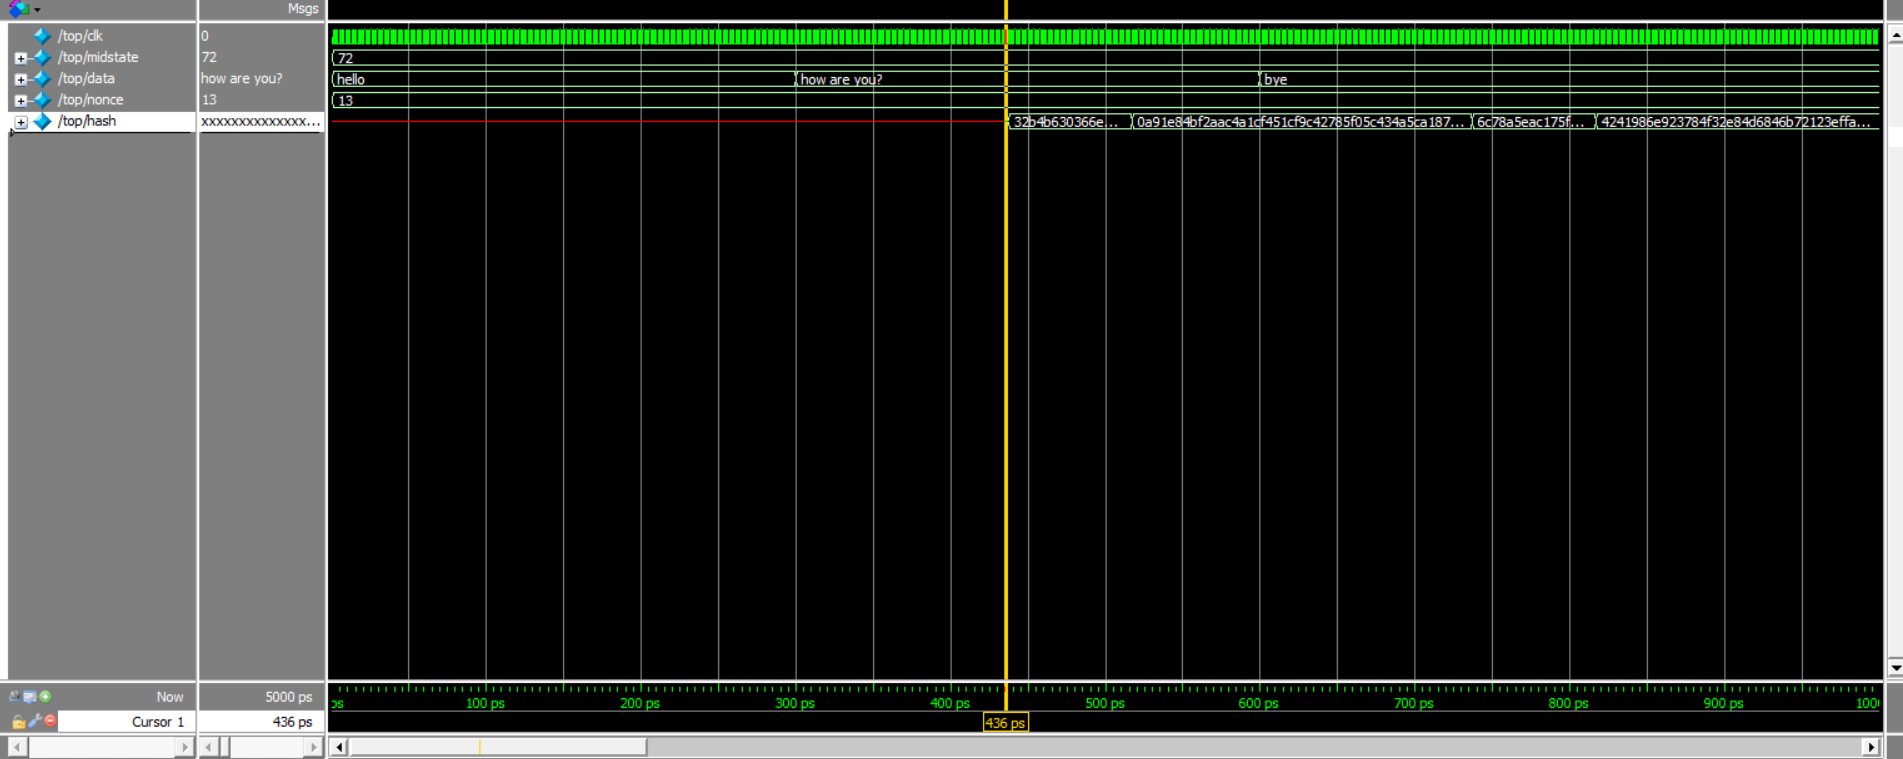
\includegraphics[width = \textwidth]{figs/simulation/1.png}
	\caption{شبیه‌سازی با \lr{Testbench}}
	\label{simulation_1}
\end{figure}

\subsection{جدول ورودی‌ها و خروجی‌های  Testbench}
\lr{
	\begin{table}[H]
		\resizebox{\textwidth}{!}{%
			\begin{tabular}{@{}llll@{}}
				\toprule
				Midstate & Nonce   & Data                                    & Time (clk)  \\ \midrule
				0        & 0       & 0                                       & 1000 - 0    \\
				96'd456  & 32'd453 & 512'd12345609823                        & 2000 - 1000 \\
				96'd456  & 32'd453 & 512'd7659432094555543122297600000000654 & End - 2000  \\ \bottomrule
			\end{tabular}%
		}
		\rl{
			\caption{مقادیر ورودی‌ها و زمان }}
		\label{table_input}
	\end{table}}

\lr{
	\begin{table}[H]
		\resizebox{\textwidth}{!}{%
			\begin{tabular}{@{}ll@{}}
				\toprule
				Hash                                                                                        \\ \midrule
				\begin{tabular}[c]{@{}l@{}}ab5283d68df053ac62d053789d4b45b81a02c959d7cab97fc43451166351f117 \\ f949fe918475f762ba80567046338211461648316d4432e6c505edc3b5ee6ff5\end{tabular} & 1217 - 433        \\
				\begin{tabular}[c]{@{}l@{}}dd477bfb0f07e299560b050c7aedb947bad77571f9a7d886a06f197a55f7946b \\ 8a9cecbb948a5478380168f8bfaf8e6d7d828459564973272b18cdf99d0234f2\end{tabular} & 1436 - 1217       \\
				\begin{tabular}[c]{@{}l@{}}0c0dea4dfd9994c6eb97f500589565239347be8a5b2e4ce4832c6cc9095baa51 \\ bf2bdde45ef619f4086e71e7d86f637314357e6d20632c31612f5424644cc223\end{tabular} & 2217 - 1436       \\
				\begin{tabular}[c]{@{}l@{}}6d383e0cceb223c20c45b816a165072ad200b8091682e8e5c31295ee62ca3719 \\ afbd493a4b85859d1cbe08d98bf01e66be18f3d3536987eeef06cc7965851bf8\end{tabular} & 2437 - 2217       \\
				\begin{tabular}[c]{@{}l@{}}6b722c1b1fb150c850e02ee44e03a447401ca4ac3cde4de6eb95b2e853d0d34b \\ 53583685f4b21f9b98229734756d7b835e46c2f589e461ab7c3177fb7e572b64\end{tabular} & End - 2437        \\ \bottomrule
			\end{tabular}%
		}
		\rl{
			\caption{مقادیر درهم‌سازی و زمان }}
		\label{table_hash}
	\end{table}}

\section{اجرا و تحلیل کد نرم‌افزاری (مدل طلایی)}
به همراه پروژه کد C الگوریتم Skein نیز به عنوان مدل طلایی ارائه شد، در ادامه مختصرا کد C مدل طلایی را تحلیل می‌کنیم.
\subsection{تحلیل کد C}
تابع $skeinhash$ با گرفتن ورودی $data$ که به صورت آرایه ای از $unsigned char$  و $output$ که به صورت آرایه‌ای از  $uint8\_t$ میباشد شروع می کند.با فراخواندن $sph\_skein512\_init$ که ورودی از جنس $sph\_skein\_big-contex$ می گیرد و سپس $sph\_skein512$ که ورودی $sph\_skein\_big-contex$ و داده و طول داده را می گیرد و در آخر $sph\_skein512\_close$ که خروجی و $sph\_skein\_big-context$ را به عنوان ورودی دارد کار خود را پایان می دهد و نتیجه را در آرایه خروجی به طول ۳۲ کپی می‌کند.\\
	در ابتدا $sph\_skein\_big-context$ بررسی می شود:
	زمینه ای برای محاسبه ی اسکین شامل مقادیر واسطه و بخشی از داده از آخرین بلوک وارد شده است.
\begin{ccode}
#ifndef DOXYGEN_IGNORE
	unsigned char buf[64];    /* first field, for alignment */
	size_t ptr; 
	sph_u64 h0, h1, h2, h3, h4, h5, h6, h7;
	sph_u64 bcount;
#endif
} sph_skein_big_context;
\end{ccode}
\begin{itemize}
\item
$buf$\\ آرایه ای به طول ۶۴ که بخش به بخش داداه را در خود ذخیره می‌کند و روی آن پردازش انجام می‌شود.
\item
$ptr$\\ سایز بخش اشغال شده بافر
\item
$h0..h7$\\
 \item
 تعداد بلاک های داده\\$bcount$
\end{itemize}
تابع $skein\_big\_init$ مقادیر  $sph\_skein\_big-context$ که از این به بعد از آن به اختصار $ctx$ یاد میشود را مقدار دهی اولیه کرده و تمامی مقادیر آن را به جز بافر صفر می‌گذارد.\\
تابع $sph\_skein512$ بخش اصلی محاسبات را به عهده دارد.اگر سایز بافر $ctx$ خالی مانده بیشتر از طول داده باشد داده در آن کپی می‌شود.\\
سپس مقادیر $ctx$ توسط تابع $READ\_STATE\_BIG$ به روز رسانی می‌شوند و با مشخص کردن مقدار $first$ که بعدتر از آن استفاده میکند و برابر با متغیر$ first$ در $UBI$  می‌باشد با استفاده از $bcount$ زمینه که در ابتدا برابر با $0$ است ،وارد لوپ محاسبه می‌شود.\\
اگر بافر پر شده باشد، $bcount$ به علاوه یک شده و $first$  و $ptr$ صفر می‌شوند. تابع $UBI\_BIG$ با ورودی $96+first$ و $0$ فراخوانی می‌شود که همان
\lr{ The Unique Block Iteration (UBI) chaining mode}
 است که یک مقدار زنجیره ای ورودی را با یک رشته ورودی با طول اختیاری ترکیب می کند و خروجی با طول ثابت را تولید می کند.\\
.بلوک های پیام $M0$ و $M1$ و …و $M7$ هرکدام گنجایش 64 بیت داده را دارند که به ترتیب توسط  بافر$ ctx$ پر می‌شوند.\\
 مقدار $p0…p7$ مربوط به threefish که متن ساده، یک رشته از بایت های با طولی برابر با کلید، است برابر $m0..m7$ قرار می‌گیرد.\\
دو متغیر $t0$ و $t1(threefish tweak)$ با استفاده از $bcount$  که متعلق به $ctx$ است و ورودی های تابع  $UBI\_BIG$ محاسبه میشوند و تابع $TFBIG\_KINIT$با ورودی های $h0 …h7 $مربوط به $ctx$ و $t0$ و $t1$ که قبلتر محاسبه شد فراخوانی میشود که با استفاده از آن و $TFBIG\_ADDKEY$ که با هم نقش  threefish اسکین را به عهده دارند $h0..h7$ مقدار دهی میشوند.به طوری که $hn = mn \textasciicircum pn$.\\
 و این مرحله تا وقتی داده ای که در بافر نرفته باقی  مانده ادامه دارد و سپس تمامی مقادیر $ctx$ در آن نوشته میشوند.(به جز بافر)\\
 تابع  $skein\_big\_close$ چند بیت اضافی (0 تا 7) را به محاسبات فعلی اضافه میکند.خروجی را در بافر ارائه شده میریزد و به پردازش خاتمه میدهد. زمینه یا $ctx$ به طور خودکار دوباره مقدار دهی اولیه می‌شود.ورودی این تابع به جز زمینه و آرایه‌ی خروجی،تعداد بیت های اضافه $n$ و خود بیت های اضافه $ub $میباشد که خود تابع دو ورودی آخر را مشخص می‌کند.اگر $n $صفر نباشد مقدار $x$ ای با استفاده از این دو تولید میشود که$ sph\_skein512$ آن فراخوانی میشود.در این مرحله، اگر $ptr == 0$ یعنی پیام خالی است؛ در غیر این صورت، بین 1 تا 64 بایت وجود دارد که هنوز پردازش نشده اند. در هر صورت بافر باید به یک بلوک کامل پر شده با صفر تبدیل شود(مشخصه Skein می گوید که پیام خالی پوشیده شده است تا حداقل یک بلوک برای پردازش وجود داشته باشد).
  هنگامی که این بلوک پردازش شده است، این فرآیند دوباره با بلوک پر از صفر، برای خروجی (آن بلوک encoding "0"، بیش از 8 بایت و سپس با صفر پر شده) انجام می شود.


\end{document}
